\chapter{Radar Model}
\label{radar_model}
With knowledge of the detrimental effects of delay-frequency sidelobes, we seek a radar measurement technique with the high sensitivity provided by coding but without the accompanying ambiguity wrought by matched filtering. In order to proceed, it is necessary to formalize the notion of sidelobe elimination. To do this, we develop a mathematical model for radar measurements and explore how this model relates to actual physical targets.

\section{Defining the Model}
\label{radar_model_definition}
\subsection{Image Blur Analogy}
Radar coding ambiguity is similar in effect to the blurring of images. Suppose there is a true image that we want to capture, $h[n,p]$. In capturing the image, the physical optics impose a point-spread function $\chi_s[n,p;n',p']$ that causes any point in the true image to be spread out in a determinable pattern in the measured image. The resulting blurred image could appear like in the example in Figure \ref{fig:image_blurring}.
\begin{figure}[tpb]
 \centering
 \begin{subfigure}[b]{0.35\textwidth}
  \centering
  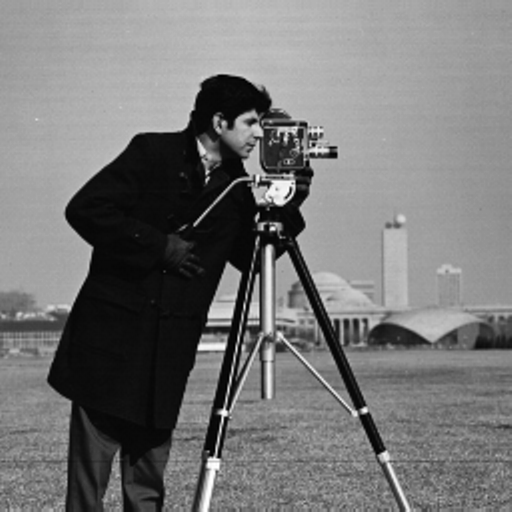
\includegraphics[width=\textwidth]{blurred_image_example_orig}
  \caption{Source image\\$h[n,p]$}
  \label{fig:source_image}
 \end{subfigure}
 \hfill
 \begin{subfigure}[b][0.35\textwidth+2\baselineskip]{0.26\textwidth}
  \centering
  \vfill
  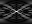
\includegraphics[width=\textwidth]{blurred_image_example_kernel}%
  \captionsetup{justification=centering}
  \vfill
  \caption{Point-spread function\\$\chi_s[n,p;N/2,L-1]$}
  \label{fig:point_spread_function}
 \end{subfigure}
 \hfill
 \begin{subfigure}[b]{0.35\textwidth}
  \centering
  
\includegraphics[width=\textwidth]{blurred_image_example_blurred}
  \caption{Blurred image\\$u[n',p']$}
  \label{fig:blurred_image}
 \end{subfigure}
 \caption[Image blurring example]{\emph{Image blurring example.} A blurred image \textbf{(\subref{fig:blurred_image})} is formed by an inner product between a source image \textbf{(\subref{fig:source_image})} and a point-spread function \textbf{(\subref{fig:point_spread_function})}. The point-spread function describes how a block of neighboring pixels in the source image is weighted and combined to get a single pixel value in the blurred image. Because the point-spread function is shift invariant in this case, the inner product amounts to a two-dimensional convolution.}
 \label{fig:image_blurring}
\end{figure}%
Mathematically, this type of blurring takes the form of an inner product between the source image $h[n,p]$ and the point-spread function $\chi_s[n,p;n',p']$:
\begin{equation}\label{eq:image_blurring}
 u[n',p'] = \innerprod[\Big]{h[n,p]}{\chi_s[n,p;n',p']} = \sum_{p=0}^{P-1} \sum_{n=0}^{N-1} h[n,p] \chi_s^*[n,p;n',p'],
\end{equation}
where $\innerprod{\cdot}{\cdot}$ denotes an inner product (two-dimensional over the $n$ and $p$ indices in this case) and $u[n',p']$ is the resulting blurred image.

In terms of the radar analogy, the resulting image $u[n',p']$ is the output of matched filtering performed on the received signal, the point-spread function $\chi_s[n,p;n',p']$ is the ambiguity function, and the source image $h[n,p]$ is the reflectivity of the target scene. The matched filter bank result was originally defined in Section \ref{matched_filtering}; it is calculated from the received signal $y[m]$ according to
\begin{equation}\label{eq:matched_filtering_for_model}
 u[n',p'] = \sum_{m=0}^{M-1} s^*[m - p' + L-1]\, e^{-2\pi i n' (m-p'+L-1)/N}\, y[m],
\end{equation}
where $s[l]$ represents the transmitted waveform and $y[m]$ represents the received signal. The ambiguity function $\chi_s[n,p;n',p']$ for the code $s[l]$ was also defined earlier, in Section \ref{radar_ambiguity}; it describes how matched filtering takes a point in delay-frequency space and spreads it into sidelobes:
\begin{multline}
 \chi_s[n,p;n',p'] = \sum_{m=0}^{M-1} s[m - p' + L - 1]\, e^{2\pi i n' (m-p'+L-1)/N}\\
 \times s^*[m - p + L - 1]\, e^{-2\pi i n (m-p+L-1)/N}.
\end{multline}
The target reflectivity $h[n,p]$ is something we have not yet encountered; it is a matrix of complex numbers that represents the magnitude and phase of the reflected signal (including the power gains and losses described by the radar equation \eqref{eq:radar_equation}) as indexed by delay $p$ and frequency $n$. In this way it is very much like a complex-valued image of delay-frequency space. Substituting these representations into the blurring equation, \eqref{eq:image_blurring}, will allow us to define a mathematical radar model.

\subsection{Ambiguity Equation}
First, though, it is convenient to simplify these equations by assigning an operator name, $A^*$, to matched filtering. By defining $A^*$ as
\begin{equation}
 A^*(y)[n,p] = \frac{1}{\sqrt{N}} \sum_{m=0}^{M-1} s^*[m - p + L-1]\, e^{-2\pi i n (m-p+L-1)/N}\, y[m],
\end{equation}
equation \eqref{eq:matched_filtering_for_model} can be written compactly as
\begin{equation}\label{eq:matched_filtering_with_operator}
 u[n',p'] = \sqrt{N} A^*\paren[\big]{y[m]}.
\end{equation}
As the notation indicates, $A^*$ is a function that takes a one-dimensional vector of length $M$ and produces a two-dimensional matrix with indices $n$ and $p$ of lengths $N$ and $P$. The matched filter operator also has an adjoint or conjugate transpose, $A$, defined by the inner product identity:
\begin{align}
 \innerprod[\Big]{A(x)}{y[m]} &= \innerprod[\Big]{x[n,p]}{A^*(y)}.
 %&= \frac{1}{\sqrt{N}} \sum_{p=0}^{P-1} \sum_{n=0}^{N-1} \brak*{x[n,p] \cdot \paren*{\sum_{m=0}^{M-1} s^*[m - p + L-1]\, e^{-2\pi i n (m-p+L-1)/N}\, y[m]}^*}\\
 %&= \frac{1}{\sqrt{N}} \sum_{m=0}^{M-1} \brak*{\paren*{\sum_{p=0}^{P-1} \sum_{n=0}^{N-1} s[m - p + L-1]\, e^{2\pi i n (m-p+L-1)/N} x[n,p]} \cdot y^*[m]}
\end{align}
From this, we can write $A$ on its own as
\begin{equation}
 A(x)[m] = \frac{1}{\sqrt{N}} \sum_{p=0}^{P-1} \sum_{n=0}^{N-1} s[m - p + L-1]\, e^{2\pi i n (m-p+L-1)/N}\, x[n,p].
\end{equation}
Again following the notation, $A$ is a function that takes a two-dimensional matrix as its argument and produces a one-dimensional vector indexed by $m$. The scaling factor of $1/\sqrt{N}$ is included in the definitions for both $A^*$ and $A$ because it ensures that the compound operator $AA^*(y)$ is the identity scaled by $\norm{2}{s}^2$. Accordingly, it is convenient to define scaled reflectivity coefficients $x[n,p]$ as
\begin{equation}
 x[n,p] = \sqrt{N} h[n,p] \quad \Leftrightarrow \quad h[n,p] = \frac{1}{\sqrt{N}} x[n,p].
\end{equation}

The measurement ambiguity equation can be formed by substituting the radar representations for the image blurring terms back into equation \eqref{eq:image_blurring}:
\begin{align}
 \sqrt{N} A^*\paren[\big]{y[m]}
 &= \begin{multlined}[t]
     \sum_{p=0}^{P-1} \sum_{n=0}^{N-1} \frac{1}{\sqrt{N}} x[n,p] \sum_{m=0}^{M-1} s^*[m - p' + L - 1]\, e^{-2\pi i n' (m-p'+L-1)/N}\\
     \times s[m - p + L - 1]\, e^{2\pi i n (m-p+L-1)/N}
    \end{multlined}\nonumber\\
 &= \begin{multlined}[t]
     \sum_{m=0}^{M-1} s^*[m - p' + L - 1]\, e^{-2\pi i n' (m-p'+L-1)/N}\\
     \times \frac{1}{\sqrt{N}} \sum_{p=0}^{P-1} \sum_{n=0}^{N-1} s[m - p + L - 1]\, e^{2\pi i n (m-p+L-1)/N}\, x[n,p].
    \end{multlined}\\
\intertext{Further simplification is possible by writing the right-hand side in terms of the $A$ and $A^*$ operators:}
 A^*\paren[\big]{y[m]}
 &= \frac{1}{\sqrt{N}} \sum_{m=0}^{M-1} s^*[m - p' + L - 1]\, e^{-2\pi i n' (m-p'+L-1)/N} A\paren[\big]{x[n,p]}\nonumber\\
 &= A^*\paren*{A\paren[\big]{x[n,p]}}.
\end{align}
We call this the ambiguity equation since it relates the ambiguous matched filter output to the artifact-free reflectivity coefficients, and the composed operator $A^*A$ completely describes the resulting delay-frequency sidelobes. Since it is easy to overlook, note that we now have the following definitions in terms of the operators $A$ and $A^*$:
\begin{align}
 \text{Matched filter bank applied to $y$:} \quad & \sqrt{N} \cdot A^*\paren{y}\label{eq:mf_Astar}\\
 \text{Ambiguity function centered at ($n_0 , p_0$):} \quad & N \cdot A^*A\paren*{\delta_{n_0,p_0}}\label{eq:ambiguity_AstarA},
\end{align}
where $\delta_{n_0,p_0}[n,p]$ is the discrete delta function that returns 1 at [$n_0 , p_0$] and 0 otherwise.

\subsection{The Radar Model}
The ambiguity equation is close to what we desire for a radar model, but one further simplification can be made. Since both sides of the equation have matched filtering applied to them, $A^*$ can be removed to arrive at a measurement equation:
\begin{equation}\label{eq:radar_model_with_operator}
 y[m] = A\paren[\big]{x[n,p]}.
\end{equation}
The measured radar signal $y[m]$ is now just a linear function of the scaled delay-frequency target reflectivity $x[n,p]$. That linear function, $A$, is the radar model. Interestingly, the radar model is the adjoint, or conjugate transpose, of the matched filter bank operation. This means that while the matched filter correlates the received signal with the expected return from point targets with different delays and frequency shifts, the radar model simulates the received signal as the sum of returns from point targets with different delays and frequency shifts. Though that mirror relationship is just something of a curiosity for now, it will have importance later when it comes to solving for the target reflectivity.

The radar model equation is useful because it provides the formalism needed for eliminating delay-frequency sidelobes: one can use the measured signal and radar model to solve for the target reflectivity. As formulated, the target reflectivity is precisely the matched filter result but with sidelobes removed. Unfortunately, it is not a straightforward process to just solve for the target reflectivity. The radar model is not invertible because equation \eqref{eq:radar_model_with_operator} is under-determined, with more unknowns in the target reflectivity than equations provided by the measurements; this is a natural consequence of allowing for unknown frequency shifts. Since the system of equations is under-determined, there are an infinite number of solutions for the target reflectivity function that would satisfy the equation and match the measurements. The matched filter result is one of those solutions, but it has serious shortcomings. Finding the best solution for the target reflectivity is the subject of Part \ref{part_waveform_inversion}, where it will be shown that sparsity of the radar scene is key to eliminating sidelobes.

Fully written out, the radar model is:
\begin{align}
 y[m] &= \frac{1}{\sqrt{N}} \sum_{p=0}^{P-1} \sum_{n=0}^{N-1} s[m - p + L-1]\, e^{2\pi i n (m-p+L-1)/N}\, x[n,p] \label{eq:radar_model_x}\\
 \intertext{or equivalently}
 y[m] &= \sum_{p=0}^{P-1} \sum_{n=0}^{N-1} s[m - p + L-1]\, e^{2\pi i n (m-p+L-1)/N}\, h[n,p]. \label{eq:radar_model}
\end{align}
In the theory of vector spaces, the model $A$ is a tight frame, conceptually the equivalent of an overcomplete basis for delay-frequency space. In fact, the model is an instance of a Gabor frame with window given by the code $s$, also known as a short time Fourier transform \autocite{Mal08}. This representation can be interpreted using the notion of a grid of point targets, which is visualized in Figure \ref{fig:delay_frequency_grid}.
\begin{figure}[tpb]
 \centering
 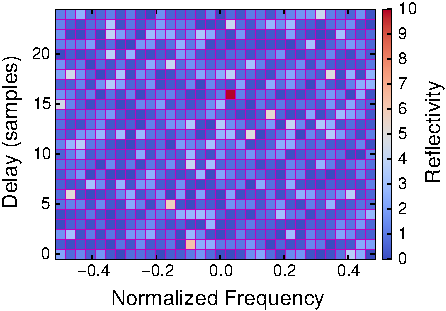
\includegraphics{range_doppler_discretization}
 \caption[Reflectivity coefficients as a delay-frequency grid of point targets]{\emph{Reflectivity coefficients as a delay-frequency grid of point targets.} Each grid point represents a location in delay-frequency space indexed by delay $p$ and frequency $n$. The color of each point corresponds to the amount of signal reflected at that particular delay and frequency shift, a value given by the magnitude of the target reflectivity coefficient $h[n,p]$. The radar scene is thus represented by a grid of independent point targets according to the radar model of equation \eqref{eq:radar_model}.}
 \label{fig:delay_frequency_grid}
\end{figure}%
The target reflectivity $h[n,p]$ can be thought to represent point targets distributed uniformly over delay-frequency space. Each point target can reflect the transmitted radar waveform independently with a given magnitude and phase. The radar model describes how reflections from each of these point targets would manifest in the measured signal, and it sums the contributions of each to produce the measurement. Again, this is just the mirror operation to what the matched filter does in its role as adjoint, assuming point targets in delay-frequency space and matching against the modeled reflection.

\section{Derivation of Radar Model}
\label{radar_model_derivation}
\subsection{Narrow-band Received Signal}
Though we now have a suitable radar model, it is instructive to derive it in another way that will allow us to relate the discrete reflectivity coefficients $h[n,p]$ to the complete reflectivity function. We begin with the narrow-band radar equation for (the complex envelope of) the baseband received signal from a fluctuating distributed target \autocite{VTre01}:
\begin{equation}
 y(t) = \int_{\rho_0}^{\rho_1} s(t - \rho) \tilde{a}\paren*{t - \frac{\rho}{2}, \rho} \dee\rho,
\end{equation}
where $s(t)$ is the transmitted baseband modulation signal and $\tilde{a}(t, \rho)$ is the complex target reflectivity (magnitude and phase) as a function of time $t$ and delay $\rho$. Note that this reflectivity function encompasses the power gained and lost according to the radar equation \eqref{eq:radar_equation}; it is not just the fraction of reflected power as described by the radar cross section $\sigma$. We have taken the integration interval to be $\brak*{\rho_0, \rho_1}$ to reflect the limited sampling window, and this carries with it the implicit assumption that $\tilde{a}(t - \rho/2, \rho) = 0$ outside that range. Whether one considers $\tilde{a}(t, \rho)$ to be random or deterministic does not matter at present. To ease further derivation, we define a new function
\begin{equation}
 \tilde{h}(t, \rho) = \tilde{a}\paren*{t + \frac{\rho}{2}, \rho}
\end{equation}
so that the time variable represents the scattering for a signal \emph{sent} at time $t$ (which arrives at the target at $t + \rho/2$) rather than one reaching the target at time $t$. This results in
\begin{equation}\label{eq:continuous_measurement}
 y(t) = \int_{\rho_0}^{\rho_1} s(t - \rho) \tilde{h}(t - \rho, \rho) \dee\rho.
\end{equation}

\subsection{Discretization}
The next step is to begin discretizing the model. We assume that the received signal is sampled at a uniform rate $\tau_s$ starting at time $t_0$ and ending at $t_1$ (inclusive), so that $y(t)$ is represented by a complex discrete sequence
\begin{align}
 y[m] = y(m\tau_s + t_0) && m = 0,\dotsc,M-1 && M = (t_1 - t_0)/\tau_s + 1.
\end{align}
In addition, we restrict our attention to discrete phase-modulated signals with $L$ bauds and a baud length of $\tau_b$, so that
\begin{equation}
 s(t) = s[l]\quad \text{for}\quad l\tau_b \le t < (l + 1)\tau_b, \quad l = 0,\dotsc,L-1
\end{equation}
for a complex sequence $s[l] \in \field{C}$. For ease of notation, let us also infinitely extend the sequence $s[l]$ by letting its value for non-existent indices be zero, $s[l] = 0$ for $l \ne 0,\dotsc,L-1$. If we assume that the sampling time is an integer multiple of the baud length, then we have $\tau_s = R\tau_b$ where $R$ is the under-sampling ratio. Note that if the reverse is true and over-sampling by an integer ratio is performed, we can simply duplicate the modulation sequence by the over-sampling ratio and let $R=1$. Finally, the time interval $[t_0, t_1]$ can be chosen to correspond to the delay interval $[\rho_0, \rho_1]$ by requiring $t_0 = \rho_0 + L\tau_b$ and $t_1 = \rho_1$. This shrinks the sampling window to ensure that all returns from outside of the delay window have no contribution to the samples (each delay affects multiple later measurements because of the length of the code). Because of this relationship, we know that the delay integration window can be divided into $(\rho_1 - \rho_0)/\tau_b = R(M-1) + L \equiv P$ equal segments of size $\tau_b$. With these assumptions, we can break up the integral in equation \eqref{eq:continuous_measurement} as follows:
\begin{align}\label{eq:discrete_transmission}
 y[m] &= y(m\tau_s + t_0)\nonumber\\
 &= \int_{\rho_0}^{\rho_1} s(m\tau_s + t_0 - \rho) \tilde{h}(m\tau_s + t_0 - \rho, \rho) \dee\rho\nonumber\\
 &= \sum_{p=0}^{RM+L-R-1} \int\limits_{\rho_0 + p\tau_b}^{\rho_0 + (p+1)\tau_b} s(Rm\tau_b + L\tau_b + \rho_0 - \rho) \tilde{h}(Rm\tau_b + L\tau_b + \rho_0 - \rho, \rho) \dee\rho\nonumber\\
 &= \sum_{p=0}^{P-1} s[Rm-p+L-1] \int\limits_{p\tau_b}^{(p+1)\tau_b} \tilde{h}(Rm\tau_b + L\tau_b - \rho, \rho + \rho_0) \dee\rho.
\end{align}

\subsection{Simplification}
Now comes a key observation: $s(t)$ is nonzero only over $0 \leq t < L\tau_b$, and $\tilde{h}(t, \rho)$ is evaluated over the same values in equation \eqref{eq:continuous_measurement}. Thus, the result of the model will be the same if we replace $\tilde{h}(t, \rho)$ with its Fourier series representation on the interval $0 \leq t \leq N\tau_b$, where $N \geq L$ and $\nu_0 = 1/(N\tau_b)$ is the smallest frequency component. The Fourier series is given by
\begin{equation}
 \tilde{h}(t, \rho) = \sum_{k = -\infty}^{\infty} h_k(\rho) e^{2\pi i k \nu_0 t} \quad \text{for} \quad 0 \leq t \leq 1/\nu_0,
\end{equation}
where
\begin{equation}\label{eq:fourier_series_coefficients}
 h_k(\rho) = \nu_0 \int_{0}^{1/\nu_0} \tilde{h}(t, \rho) e^{-2\pi i k\nu_0 t} \dee t
\end{equation}
defines the Fourier coefficients. Substituting the Fourier series representation into equation \eqref{eq:discrete_transmission} yields
\begin{multline}
 y[m] = \sum_{p=0}^{P-1} s[Rm-p+L-1]\\
 \times \int\limits_{p\tau_b}^{(p+1)\tau_b} \sum_{k = -\infty}^{\infty} h_k(\rho + \rho_0) e^{2\pi i k(Rm + L)/N} e^{-2\pi i k\nu_0 \rho} \dee\rho.
\end{multline}
This seems to have made the model more complicated for no benefit: there are now three discrete parameters and an infinite sum to boot. Notice, however, that $e^{2 \pi i k(Rm+L)/N}$ as a function of $k$ is periodic with period $N$. Re-parameterizing the infinite sum leads to
\begin{multline}
 y[m] = \sum_{p=0}^{P-1} s[Rm-p+L-1] \\
 \times \sum_{n=0}^{N-1} e^{2 \pi i n(Rm+L)/N} \int\limits_{p\tau_b}^{(p+1)\tau_b} \sum_{k = -\infty}^{\infty} h_{n + kN}(\rho + \rho_0) e^{-2\pi i (n + kN) \nu_0 \rho} \dee\rho.
\end{multline}
Now the result of the integral is indexed by $n$ and $p$ where $n$ parameterizes the frequency domain and $p$ parameterizes the delay domain. However, it doesn't quite match the earlier radar model definition in equation \eqref{eq:radar_model}. Factoring out the required terms produces
\begin{multline}
 y[m] = \sum_{p=0}^{P-1} \sum_{n=0}^{N-1} s[Rm-p+L-1] e^{2 \pi i n(Rm-p+L-1)/N}\\
 \times e^{2 \pi i n(p+1)/N} \int\limits_{p\tau_b}^{(p+1)\tau_b} \sum_{k = -\infty}^{\infty} h_{n + kN}(\rho + \rho_0) e^{-2\pi i (n + kN) \nu_0 \rho} \dee\rho.
\end{multline}
The form of this equation matches, and thus we define the discrete reflectivity coefficients as
\begin{equation}\label{eq:reflectivity_coefficients_not_simplified}
 h[n,p] = e^{2 \pi i n(p+1)/N} \int\limits_{p\tau_b}^{(p+1)\tau_b} \sum_{k = -\infty}^{\infty} h_{n + kN}(\rho + \rho_0) e^{-2\pi i (n + kN) \nu_0 \rho} \dee\rho
\end{equation}
and arrive once again at the discrete linear radar model:
\begin{equation}\label{eq:radar_model_with_R}
 y[m] = \sum_{p=0}^{P-1} \sum_{n=0}^{N-1} s[Rm-p+L-1] e^{2 \pi i n(Rm-p+L-1)/N} h[n,p].
\end{equation}
The only difference this time is the generalization to include undersampling of the transmitted waveform by a factor of $R$.

\subsection{Assumptions}
To sum up the derivation, recall the assumptions that underpin this model. We started with the narrow-band radar equation, which assumes that the bandwidth of the signal is much smaller than the baseband frequency so that the Doppler effect can be approximated only by frequency shifts and not time dilation. We also made the standard assumption that there is no scattering from outside the ranges parametrized by the model. In terms of the discretization, we assumed that the received signal is uniformly sampled at a fixed rate and that the transmitted waveform is piecewise constant over uniform intervals. We also required a uniformly-spaced frequency index with a number of frequency steps $N$ greater than the number of bauds $L$ in the transmitted waveform. All of these assumptions are congruous with standard radar practices and none are overly restrictive. From this we get an exact representation of the complete target reflectivity function as a discrete set of reflectivity coefficients $h[n,p]$.

\section{Representation of Targets}
\label{radar_model_representation}
\subsection{Deterministic Reflectivity}
The radar model allows us to analyze measurements in terms of delay-frequency reflectivity coefficients $h[n,p]$, but it is unclear as of yet how these coefficients embody actual radar target scenes. It is easy to think of the coefficients as representing a grid of point targets with different delays and frequency shifts, but this is highly unlikely to be the physical reality. Fortunately, the radar model derivation provides an exact relationship between the reflectivity coefficients and the complete reflectivity function, equation \eqref{eq:reflectivity_coefficients_not_simplified}, that we can use to provide an intuitive interpretation. As shown in Appendix \ref{reflectivity_coefficients}, the reflectivity coefficient equation can be simplified to
\begin{align}\label{eq:reflectivity_coefficients}
 h[n,p] = \int\limits_{p\tau_b}^{(p+1)\tau_b} \brak*{h(f, \rho + \rho_0) e^{-2\pi i f (\rho - (p+1)\tau_b)} * b_{N,\tau_b}(f)}\!(n\nu_0) \dee\rho,
\end{align}
where the new term $b_{N,\tau_b}(f)$ is a frequency-blurring kernel involving the periodic sinc function. This kernel is defined as
\begin{align}
 b_{N,\tau_b}(f) &= e^{-\pi i \tau_b f (N-1)} \mathrm{psinc}_N(2\pi \tau_b f)\\
 &= \frac{1}{N} e^{-\pi i \tau_b f (N-1)} \frac{\sin(\pi N \tau_b f)}{\sin(\pi \tau_b f)},
\end{align}
and the periodic sinc function $\mathrm{psinc}_N(2\pi \tau_b f)$ is plotted in Figure \ref{fig:periodic_sinc} for reference.
\begin{figure}[tpb]
 \centering
 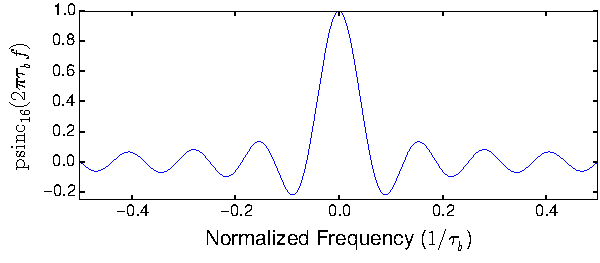
\includegraphics{periodic_sinc}
 \caption[Periodic sinc]{\emph{Periodic sinc.} The periodic sinc function, shown here for $N=16$, results from taking the discrete-time Fourier transform of the $N$-sample wide rect function. It is periodic over the width of the displayed frequency window, $1/\tau_b$.}
 \label{fig:periodic_sinc}
\end{figure}%
If the reflectivity function $h(f, \rho)$ is taken to be deterministic, the interpretation of equation \eqref{eq:reflectivity_coefficients} is straightforward: in the Doppler frequency variable $n$, the coefficients represent samples from the reflectivity function frequency spectrum $h(f, \rho)$ after it has been "smeared" by $b_{N,\tau_b}(f)$ through convolution; in the time delay variable $p$, the coefficients represent an integration of the reflectivity function over the corresponding delay window.

\subsection{Probabilistic Reflectivity}
Concerning the more general case of a probabilistic reflectivity function, we invoke the doubly-spread target model of \textcite{VTre01}: assume that the reflectivity function $h(f, \rho)$ is a zero-mean complex Gaussian random variable with autocovariance given by
\begin{equation}
 \mathrm{E}\brak*{h(f, \rho) h^{*}(f', \rho')} = S(f, \rho) \delta(f - f') \delta(\rho - \rho'),
\end{equation}
where $\mathrm{E}[\cdot]$ denotes expected value and $S(f, \rho)$ is the scattering function describing the returned \emph{power} as a function of frequency and range. The process is zero-mean because the phase of $h(f, \rho)$ is assumed to follow a uniform distribution that is independent of the magnitude. In practical terms, the main difference between the deterministic model and the doubly-spread model is the phase of the returned signal: the former model produces phases that are a fixed function of range, while the latter model produces random phases with respect to range. Which of these is appropriate will depend upon the application; the deterministic model is best for simple targets with a known form, while the probabilistic model is best for targets that vary over time or present upredictably complex scattering. Fortunately, both formulations fit equally well with the radar model. In terms of the reflectivity coefficients, the doubly-spread target model results in
\begin{equation}\label{eq:reflectivity_coefficients_doubly_spread}
 \mathrm{E}\brak*{h[n,p]h^*[n,p]} = \int\limits_{p\tau_b}^{(p+1)\tau_b} \brak*{S(f, \rho + \rho_0) * B(f)}\!(n\nu_0) \dee\rho
\end{equation}
with
\begin{align}
 B(f) &= \mathrm{psinc}_N^2(2\pi \tau_b f)\\
 &= \frac{1}{N^2} \frac{\sin^2(\pi N\tau_b f)}{\sin^2(\pi \tau_b f)}.
\end{align}
In this case, the relationship between the coefficients and the actual quantity of interest $S(f, \rho)$ is even clearer: on average, the coefficients $\abs[\big]{h[n,p]}^2$ give the total power returned by the target from ranges $p\tau_b \le \rho - \rho_0 < (p+1)\tau_b$ and frequencies weighted by the squared periodic sinc $B(n\nu_0 - f)$. Both the deterministic and doubly-spread target models lead to similar interpretations for the reflectivity coefficients; the difference is in how the phases of the returned signals add up.

\subsection{Reflectivity Coefficient Sparsity}
\label{point_target_reflectivity}
With the deterministic and probabilistic interpretations of the reflectivity coefficients in hand, we can finally address a matter of vital importance: under what conditions are the reflectivity coefficients sparse? Recall that radar scenes are typically sparse, with scatterers occupying only a small portion of delay-frequency space. Thus, the complete reflectivity function $h(f, \rho)$ can be assumed to have sparse support. The hope is that this sparsity translates into sparsity of the reflectivity coefficients. If it does, we can use that prior knowledge to find the sparsest solution for $h[n,p]$ that matches the measurements according to the radar model and have confidence that it is the true sidelobe-free solution.

To illustrate the reflectivity coefficient interpretations and analyze the coefficient sparsity for the sparsest possible target, consider the case of a point target with a reflectivity of $A$ initially at range $r$ and traveling toward the radar with a range rate $v$. The target's time delay and Doppler frequency shift are given by $\rho_t \approx \frac{2r}{c}$ and $f_t \approx \frac{2v}{c}f_0$ respectively, where $c$ denotes the speed of light and $f_0$ is the baseband radar frequency. The appropriate target reflectivity function is
\begin{align}
 \tilde{h}(t, \rho) &= A e^{2\pi i f_t t} \delta(\rho - \rho_t) e^{2\pi i f_t \rho} e^{-2\pi i f_0 \rho_t}\\
\intertext{or equivalently}
 h(f, \rho) &= A \delta(f - f_t) \delta(\rho - \rho_t) e^{2\pi i f_t \rho} e^{-2\pi i f_0 \rho_t}.
\end{align}
Plugging this into equation \eqref{eq:reflectivity_coefficients} shows how the discrete model represents a point target:
\begin{equation}
 h[n,p] = \begin{cases}
            A\, b_{N,\tau_b}(n\nu_0 - f_t) e^{2\pi i f_t(\rho_0 + (p+1)\tau_b)} e^{-2\pi i f_0 \rho_t} & p = p_t\\
            0 & p \neq p_t,
           \end{cases}
\end{equation}
where $p_t$ gives the delay index which satisfies $p_t\tau_b \leq \rho_t - \rho_0 < (p_t+1)\tau_b$. In order to look at sparsity, it will be easier to visualize the magnitude of the reflectivity coefficients. This is given by
\begin{equation}\label{eq:point_target_coefficients}
 \abs[\Big]{h\brak[\big]{n,p_t}} = \frac{A}{N} \abs*{\frac{\sin\paren[\big]{\pi N\tau_b (n\nu_0 - f_t)}}{\sin\paren[\big]{\pi\tau_b (n\nu_0 - f_t)}}}.
\end{equation}
Example point target reflectivity coefficients given by equation \eqref{eq:point_target_coefficients} are shown in Figure \ref{fig:point_target_coefficients}.
\begin{figure}[tpb]
 \centering
 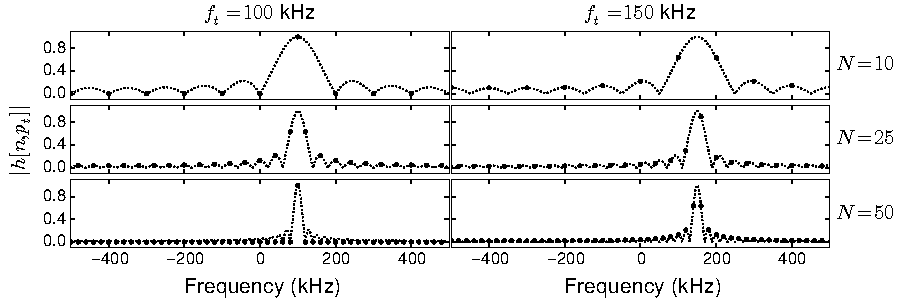
\includegraphics{point_target_coefficients}
 \caption[Reflectivity coefficients for point targets]{\emph{Reflectivity coefficients for point targets.} The reflectivity coefficient magnitudes are given by equation \eqref{eq:point_target_coefficients} with $A = 1$ and $\tau_b = 1 \, \mu\textrm{s}$ as a function of frequency for six point target cases. The left column shows the values for a point target with Doppler frequency shift of 100 kHz, while the right column shows values for a Doppler shift of 150 kHz. The first row shows the coefficient values when 10 frequencies are included in the discrete model, the second row shows values for 25 frequencies, and the third row shows values for 50 frequencies. The dotted line in each plot shows the underlying curve from which the coefficients are sampled.}
 \label{fig:point_target_coefficients}
\end{figure}%
Notice that if $n_t\nu_0 = f_t$ for some integer $n_t$, then all of the coefficients are zero except for $h[n_t,p_t]$ and target sparsity translates directly into coefficient sparsity. However, in general all of the frequency coefficients corresponding to the correct range will be nonzero, and the question then becomes one of degree: are there few enough significant coefficients to say that they are sparse? In practical terms, "significant" means being above the noise level, since smaller values can be taken as zero and the reconstruction error will still be acceptable.

Figure \ref{fig:point_target_coefficients} suggests one way of ensuring that the coefficient sparsity emulates the reflectivity function sparsity for point targets and by extension any general target: increasing $N$, the number of frequencies included in the discrete model. As $N$ increases, the discretization effects become more localized and the values $h[n,p_t]$ for the point target look more like direct frequency samples from $h(f, \rho_t)$. This is a consequence of the frequency-smearing interpretation of the relationship between the reflectivity function and coefficients. Since the periodic sinc becomes more delta-like as $N$ increases, the smearing it produces decreases. It is important to note that this is the same problem and solution encountered when relating the discrete Fourier transform of a sampled function to the complete function's Fourier transform. So we conclude that in general with $N$ large enough, sparsity of $h(f, \rho)$ for any target translates directly to sparsity of $h[n,p]$.